\chapter{Evolução de Projetos de Software}

Este trabalho visa contribuir diretamente com um software livre, tratando a evolução do mesmo. Dessa forma, neste capítulo, apresentamos os principais conceitos relacionados com esse tipo de software, passando pelas definições básicas, processos de desenvolvimento e os padrões para se contribuir com um projeto de software livre. Complementarmente, discutimos o que é evolução de software, tratando as Leis de Lehman e como está apresentada na literatura os estudos sobre a evolução de projeto de software livre.

%-------------------------------------------------------------------------------


%-------------------------------------------------------------------------------

\section{Evolução de Software}

Atualmente as tecnologias da informação exercem cada vez mais influência na sociedade, seja na interação entre pessoas, ou nas relações que empresas possuem com o mercado. Empresas, que possuem parte dos seus lucros associados diretamente, ou não, há sistemas de software, precisam evolui-los, seja para adequa-los à mudanças no ambiente onde estão inseridos, ou para mante-los competitivos frente aos concorrentes. Além desses fatores, quando os sistemas em questão são desenvolvidos como softwares livres, eles também precisam evoluir para que se mantenham sempre atrativos, motivando a comunidade estabelecida ao seu redor. Sistemas estagnados desmotivam usuários ou colaboradores, o que significa risco de perda de mercado ou enfraquecimento de um projeto de software livre, já que esses são feitos de colaboradores
%[modificar esse parágrafo com base no artigo challanges_sw_evolution]

Por outro lado, a manutenção desses sistemas é difícil, consome bastante tempo e recursos. Tarefas como adicionar novas funcionalidades, suporte a novos dispositivos de hardware, correção de defeitos, entre outros, se tornam mais difíceis conforme o sistema cresce e envelhece \cite{godfrey2000evolution}.

Acima foram mencionados os termos manutenção e evolução de software. Na maioria das vezes esses palavras aparecem juntas na literatura, e embora se refiram ao mesmo fenômeno, possuem ênfases diferentes. Manutenção é o ato de manter uma entidade num estado de reparo, capacidade ou disponibilidade, prevenindo-a contra falhas, mantendo a satisfação dos envolvidos ao longo do ciclo de vida do software. Já a evolução refere-se a um processo de mudança contínuo de um estado mais baixo, simples ou pior para um estado mais alto, mais complexo e melhor, refletindo a soma de todas as alterações implementadas no sistema.

%evolução de software sempre existiu, porem nao era estudada
A evolução de software foi identificada pela primeira vez no final dos anos 60, embora não denominada evolução até 1969, quando Meir M. Lehman realizou um estudo com a IBM, com a ideia de melhorar a efetividade de programação dessa empresa. Apesar de não ter recebido tanta atenção e pouco impactado nas práticas de desenvolvimento dessa companhia , esse estudo fez surgir um novo campo de pesquisa, a evolução de software.
%\cite{Artigo IBM}.

Durante esses estudos, Lehman formulou as três primeiras, de um total de oito leis, conhecidas atualmente como leis de Lehman. O restante foi formulado em estudos posteriores, conforme a relevancia desse campo aumentava. O conjunto dessas oito leis estão listadas abaixo:
\begin{table}[H]
\begin{center}
    \begin{tabular}{ | l | p{4cm} | p{9cm} |}
    \hline
    Índice (Ano) & Nome & Descrição \\ \hline
    1 (1974) & Mudança contínua & Um software deve ser continuamente adaptado, caso contrário se torna progressivamente menos satisfatório. \\ \hline
    2 (1974) & Complexidade Crescente & À medida que um software é alterado, sua complexidade cresce, a menos que um trabalho seja feito para mantê-la ou diminuí-la. \\ \hline
    3 (1974) & Auto-regulação & O processo de evolução de software é auto-regulado próximo à distribuição normal com relação às medidas dos atributos de produtos e processos. \\ \hline
    4 (1978) & Conservação da estabilidade organizacional & A não ser que mecanismos de retro-alimentação tenham sido ajustados de maneira apropriada, a taxa media de atividade global efetiva num software em evolução tende a ser manter constante durante o tempo de vida do produto. \\ \hline
    5 (1991) & Conservação da Familiaridade & De maneira geral, a taxa de crescimento incremental e taxa crescimento a longo prazo tende a declinar. \\ \hline
    6 (1991) & Crescimento contínuo & O conteúdo funcional de um software deve ser continuamente aumentado durante seu tempo de vida para para manter a satisfação do usuário. \\ \hline
    7 (1996) & Qualidade decrescente & A qualidade do software será entendida como declinante a menos que o software seja rigorosamente adaptado às mudanças no ambiente operacional. \\ \hline
    8 (1971/96) & Sistema de Retro-alimentação & Processos de evolução de software são sistemas de retro-alimentação em múltiplos níves, em múltiplos laços (loops) e envolvendo múltiplos agentes. \\ \hline
    \end{tabular}
    \caption{Leis de Lehman, extraído de \cite{fernandez2008empirical}}
    \label{tab-leis-lehman}
\end{center}
\end{table}

Ao contrário das engenharias tradicionais, a engenharia de software tem em mãos um produto abstrato e intangível, o que resulta em alguns desafios inerentes aos processo de desenvolvimento. A evolução de software busca amenizar ou solucionar alguns desses desafios \cite{mens2005challenges}, entre eles:

\begin{itemize}
\item Manter e melhorar a qualidade do software;
\item Suportar evolução do modelo de desenvolvimento (não só código-fonte);
\item Manter consistência entre artefatos relacionados;
\item Integrar mudanças dentro do ciclo de desenvolvimento de software;
\item Necessidades de bons sistemas de controle de versão;
\item Integração e análise de dados de várias fontes (relatórios de erros, métricas, solicitações de mudança);
\end{itemize}

%importancia
Quando inserida ou considerada nos processos de desenvolvimento, ela resulta numa excelente alternativa para evitar os sintomas do envelhecimento e inconsistencias entre o próprio software e o ambinte onde está inserido \cite{mens2005challenges}.
%\subsection{Evolução de Software Livre}
%grande crescimento dos softwares livres em geral, a exemplo do linux
Dessa forma, argumentamos que o desenvolvimento de projetos de software livre têm colaborado para a produção de softwares de alta qualidade com grande número de funcionalidades. Um exemplo disso é o sistema operacional Linux, que nas últimas décadas, entre outro pontos, tem experimentado um grande sucesso comercial.

Em geral, sistemas desenvolvidos por meio de projetos de software livre tendem a crescer com o passar do tempo, após sucessivas releases. Esse comportamento sugere consistência com a sexta lei de Lehman, que se refere ao crescimento contínuo. Nesse sentido, além de um comportamento necessário para manter a satisfação do usuário, o crescimento contínuo de um software livre é importante para manter a motivação da comunidade estabelecida ao seu redor.

Por exemplo, para avaliar esse comportamento de contínuo crescimento em softwares livres, \citeonline{godfrey2000evolution} realizaram pesquisas, do tipo estudo de caso, baseados no sistema operacinal Linux.
%
A Figura \ref{fig-evolucaolinux} mostra o crescimento do sistema operacional Linux desde sua primeira release, no ano de 1994. Desde então, ele é mantido por centenas de desenvolvedores que o desenvolvem em dois ramos paralelos: stable releases contendo as principais atualizações e correções de defeitos, e \textit{development releases} com funcionalidades experimentais e porções de código não testado.

\graphicspath{{figuras/}}
\begin{figure}[H]
\centering
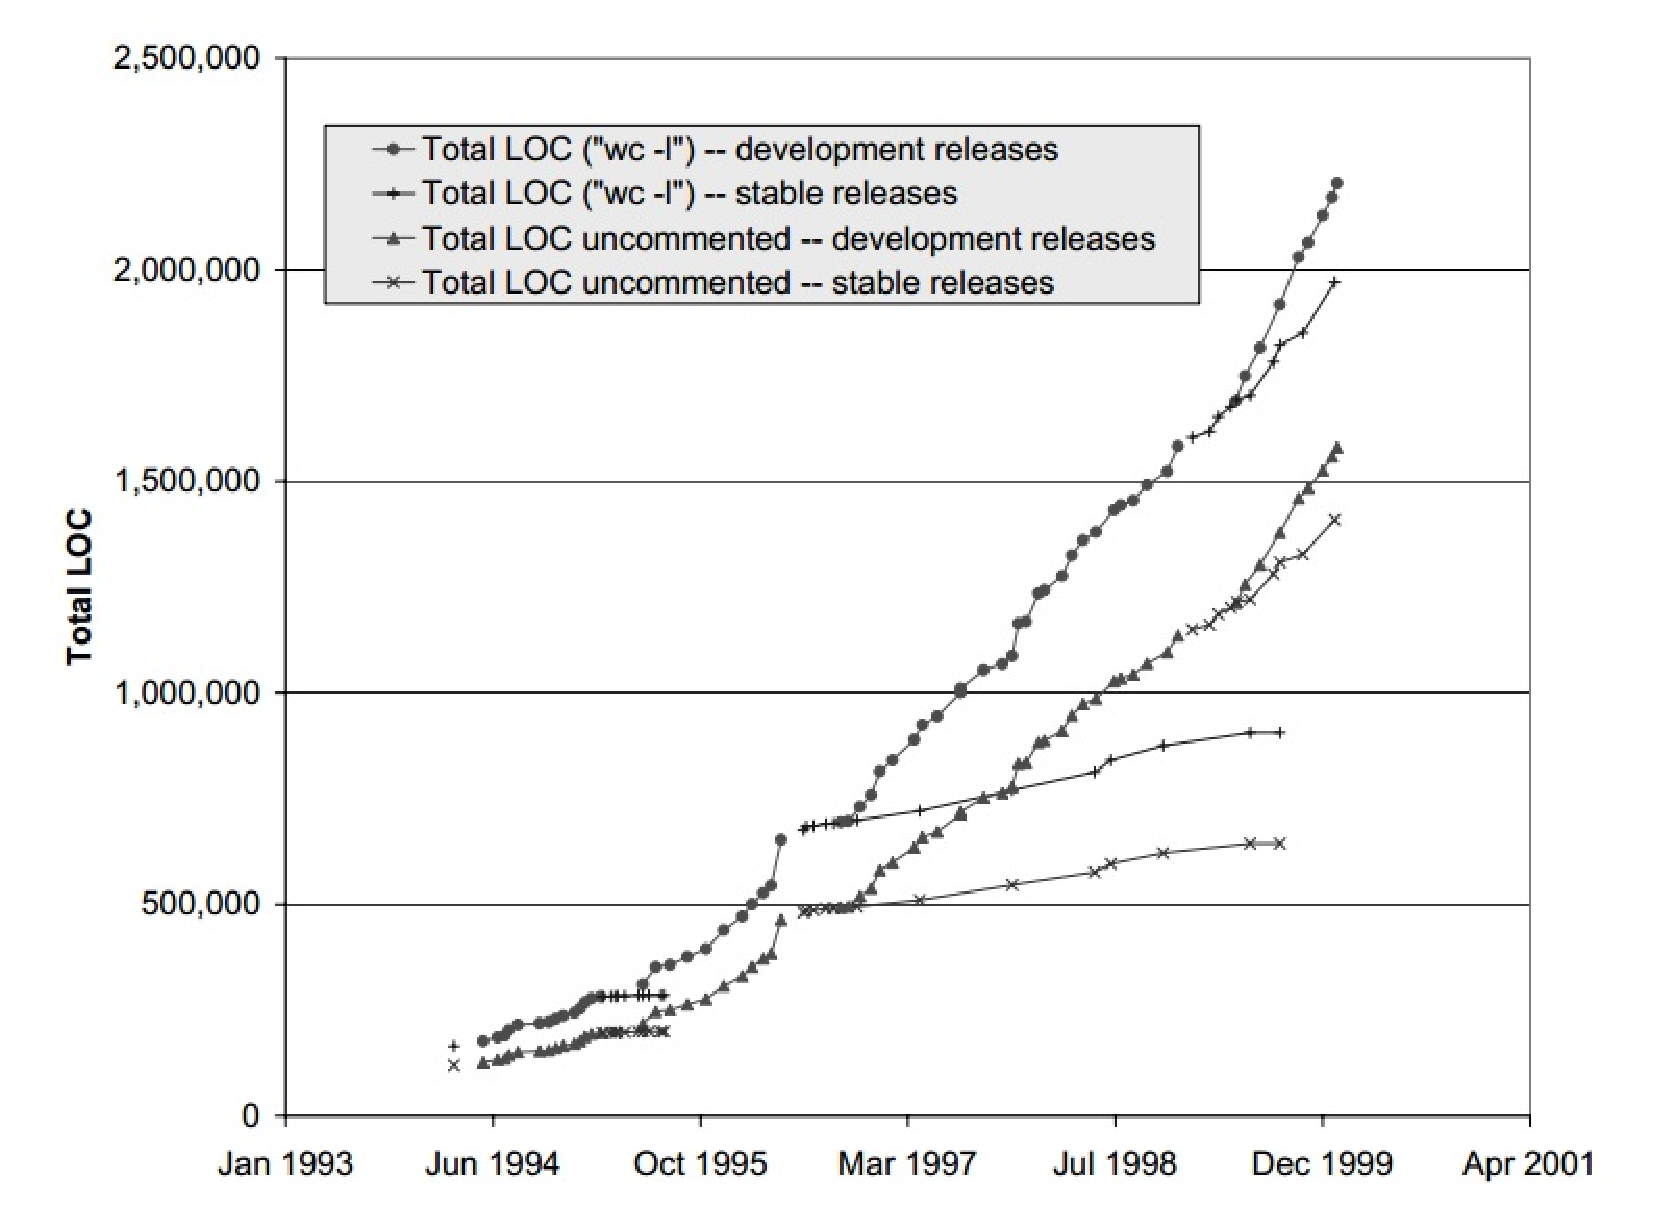
\includegraphics[width=0.6\textwidth]{linux-evolution}
\caption{Evolução do sistema operacional Linux, extraído de \cite{godfrey2000evolution}}
\label{fig-evolucaolinux}
\end{figure}

Os dados presentes no gráfico, até o início dos anos 2000, vão de encontro à quinta lei de Lehman, citada na Tabela \ref{tab-leis-lehman}. No gráfico, o número de linhas de código (LOC) do kernel do sistema, possui taxa de crescimento positiva, enquanto a lei afirma que ao longo do tempo a taxa de crescimento tende a diminuir.
%
Por outro lado, neste trabalho, não estamos tratando a evolução de software do ponto de vista da inserção de novas funcionalidades, o que pode levar ao crescrimento de número de linhas de código, como exemplificado acima. Estamos tratando a evolução de um software livre real, do ponto de vista da sua arquitetura, de acordo com as decisões julgadas pelo seus principais desenvolvedores, conforme descrito nas respostas ao questionário apresentado no Apêndice \ref{form-pesquisa}, para poderem evoluir o projeto de uma forma mais rápida e objetivando formação de uma comunidade de desenvolvedores.

\section{Processo de Desenvolvimento de Software Livre}
\label{sec-proc-sl}

O aspecto mais importante de um software livre, sob a perspectiva da Engenharia de Software é o seu processo de desenvolvimento. Um projeto de software livre começa quando um desenvolvedor individual ou uma organização decidem tornar um projeto de software acessível ao público. Seu código-fonte é licenciado de forma a permitir seu acesso e alterações subsequentes por qualquer pessoa. Tipicamente, qualquer pessoa pode contribuir com o desenvolvimento, mas mantenedores ou líderes decidem quais contribuições serão incorporadas à release oficial. Não é uma regra, mas projetos de software livre, muitas vezes, recebem colaboração de pessoas geograficamente distantes que se organizam ao redor de um ou mais líderes \cite{corbucci2011freemethods}. 

Há características presentes no software livre que, a princípio, tornam incompatível a aplicação de métodos ágeis em seu desenvolvimento, por exemplo. Entre essas características estão a distância entre os desenvolvedores e a diversidade entre suas culturas, que dificultam a comunicação, um dos principais valores dos métodos ágeis. Entretanto, o sucesso resultante de alguns projetos de software livre, como é o caso do Kernel do Linux \footnote{\url{https://www.kernel.org/}}, fizeram surgir estudos com foco na união dessas duas vertentes.

Analisando um pouco melhor projetos de software livre, é possível notar que esses compartilham princípios e valores presentes no manifesto ágil \footnote{\url{http://agilemanifesto.org/}}. Adaptação a mudanças, trabalhar com \textit{feedback} contínuo, entregar funcionalidades reais, respeitar colaboradores e usuários e enfrentar desafios, são qualidades esperadas em desenvolvedores que utilizam métodos ágeis e são naturalmente encontradas em projetos de software livre.

Num trabalho realizado, \citeonline{corbucci2011freemethods} analisa semelhanças entre projetos de software livre e métodos ágeis, através de uma relação entre os quatro valores enunciados no manifesto ágil e práticas realizadas em projetos livres. 
%
%TODO: descrever relação entre valores do manifesto ágil e práticas de projetos de software livre.
% Não precisa colocar o manifesto ágil vai direto para a relação.
% TODO: Não explicou a questão dos níveis de colaboração, desde o usuário passivo até um desenvolvedor core, exemplificando que, no momento, através deste trabalho, você é um desenvolvedor periférico.
%TODO: Reescrever com suas palavras no TCC 2 (TESE DO PAULO ABAIXO)
%
Conceitualmente, os valores semelhantes são:

\begin{itemize}

\item {Indivíduos e interações são mais importantes que processos e ferramentas.}

\item {Software em funcionamento é mais importante que documentação abrangente.}

\item {Colaboração com o cliente (usuários) é mais importante que negociação de contratos.}

\item {Responder às mudanças é mais importante que seguir um plano.}

\end{itemize}

Além disso, várias práticas disseminadas pelas metodologias ágeis são usadas no
dia-a-dia dos desenvolvedores e equipes das comunidades
de software livre~\cite{corbucci2011freemethods}:

\begin{itemize}

\item {Código compartilhado (coletivo);}
\item {Projeto simples;}
\item {Repositório único de código;}
\item {Integração contínua;}
\item {Código e teste;}
\item {Desenvolvimento dirigido por testes, e}
\item {Refatoração.}

\end{itemize}

Observar e entender esses aspectos nos projetos de software livre tornam-se
relevantes à medida que muitos projetos de software livre não vão além dos
estágios iniciais e muitos acabam sendo abandonados antes de produzir
resultados razoáveis.
%
Isso sugere que, mesmo com o sucesso de alguns projetos de software livre,
as comunidades, com ou sem a participação de empresas, podem avançar no
acompanhamento do desenvolvimento dos projetos de software livre que participam.
%
Olhar o processo de desenvolvimento de software livre do ponto de vista da 
Engenharia de Software e as possíveis sinergias com os métodos ágeis podem
contribuir para um melhor rendimento dessa disposição na criação e colaboração
em torno de projetos de software livre~\cite{meirelles2013metrics}.

Na prática, dentro do processo de desenvolvimento de software livre, após lançar
uma versão inicial e divulgar o projeto, os usuários interessados começam a
usar o software livre em questão. 
%
De acordo com Eric Raymond,``bons programas nascerem de
necessidades pessoais'', esses usuários podem também ser desenvolvedores, que
irão colaborar com o projeto a fim de atenderem às suas próprias necessidades.
%
Destacando a colaboração no código-fonte, essas melhorias são enviadas aos
mantenedores do projeto como \emph{patches}, ou seja, arquivos que
contém as modificações no código e que serão analisados pelos mantenedores que,
caso concordem com a mudança e com a sua implementação em si, irão
aplicá-las ao repositório oficial do projeto.
%
Portanto, mesmo que em projetos maiores outros aspectos sejam levados em consideração ou
sigam processos mais burocrático de colaboração, a essência da colaboração
técnica está no envio e análise de trechos de código-fonte \cite{meirelles2013metrics}.


\section{Padrões de Software Livre}
\label{sec-padroes-sl} 

Um software livre é concebido através de um processo de contribuições, o qual possui características especiais que promovem o surgimento de diversas práticas influenciadas por diversas forças. Tais práticas são conhecidas como padrões de software livre. Para simplificar, nesta seção o termo padrão está associado a padrões de software livre. Esses padrões estão organizados dentro de três grupos:

\begin{itemize}

	\item \textbf{Padrões de seleção} auxiliam prováveis colaboradores a selecionar projetos adequados.

		\begin{itemize}

			\item O primeiro padrão de seleção recomenda colaboradores novatos a "caminhar sobre terreno conhecido", ou seja, se deseja contribuir, começar por algum software que seja familiar, como por exemplo, um browser, editor de texto, IDE\footnote{Integrated Development Environment, um ambiente integrado para desenvolvimento de software}, ou qualquer outro software que já se utiliza.

			\item O segundo padrão é similar ao primeiro, porém ao invés da ferramenta ser familiar, esse padrão recomenda que o colaborador tenha conhecimentos na linguagem ou tecnologia utilizada no projeto.

			\item Já o terceiro padrão desse grupo motiva colaboradores a procurar por projetos de software livre que ofereçam fucionalidades atrativas, mesmo que o novo colaborador não tenha familiaridade com a ferramenta nem com a tecnologia utilizada em seu desenvolvimento.
		\end{itemize}

O terceiro padrão é o que melhor se encaixa ao contexto desse trabalho, já que o Mezuro não era uma ferramenta utilizada no cotidiano e tão pouco familiar. Além disso, as tecnologias utilizadas em seu desenvolvimento não eram as de maior conhecimento. Entretanto, as funcionalidades providas por essa plataforma foi determinante para essa contribuição.

	\item \textbf{Padrões de envolvimento} lidam com os primeiros passos para que o colaborador se familiarize e se envolva com o projeto selecionado.

		\begin{itemize}
			\item Entrar em contato com mantenedores para aprender sobre o contexto 	histórico e político no qual aquele projeto está inserido.

			\item Realizar instalação e checar se todo o ambiente do projeto está 	corretamente configurado em um período limitado de tempo (máximo um dia)

			\item Durante uma apresentação do sistema,  por parte de algum mantenedor, interagir para se familiarizar melhor com funcionalidades e cenários presentes no sistema.

			\item Avaliar o estado do sistema através de uma breve, mas intensa revisão de código. Isso ajuda a ter uma primeira impressão sobre a 					qualidade do código-fonte.

			\item Através da leitura, avaliar a relevancia da documentação em um 			período limitado de tempo.

			\item Checar a lista de tarefas a serem feitas. Ela pode conter bons 			pontos de partida para começar uma contribuição.

			\item Relacionado ao padrão mencionado acima, está o padrão que recomenda novos colaboradores iniciarem por tarefas mais fáceis. Começar uma tarefa 			e termina-la é importante para manter colaboradores motivados, e conforme 			ganharem mais experiencia e familiaridade com o software avançam para 			tarefas mais complexas.
	\end{itemize}

No contexto deste trabalho, muitos dos padrões desse grupo foram inseridos ao processo de contribuição. Por exemplo, o orientador deste trabalho é também mantenedor da plataforma Mezuro, assim como outros colaboradores da plataforma, auxiliaram durante o processo de envolvimento, apresentando funcionalidades e principais cenários do sistema, além de fornecer documentação necessaŕia para o entendimento do histórico e contexto no qual o Mezuro está inserido.
	
	\item \textbf{Padrões de contribuição} documenta as melhores práticas para 	se contribuir com softwares livres. Os grupos anteriores tratavam como iniciar 	e se familiarizar com um projeto de software livre. Esse grupo, por sua vez, 		contém padrões que auxiliam o fornecimento de insumos para projetos de software livre, seja codigo-fonte ou outros artefatos presentes no processo de desenvolvimento.

	\begin{itemize}

		\item Uma boa contribuição para projetos de software em geral, é a escrita de documentação. O código-fonte muitas vezes não é o suficiente para que todos os envolvidos entendam o andamento do projeto, pois apesar de promoverem o software não possuem conhecimento técnico suficiente. Além disso, documentação do projeto auxilia na manutenção e evolução do produto.

		\item Muitos softwares livres não suportam o idioma de diversos colaboradores. Um bom ponto de partida seria a internacionalização do sistema, incluindo a própria linguagem no sistema.

		\item Reportar bugs eficientemente, pois é comum que colaboradores identifiquem bugs mas ao reporta-los não são claros com respeito ao seu contexto, dificultado sua correção.

		\item Utilizar a versão correta para tarefas. Durante o desenvolvimento de software há diferentes versões, onde há no mínimo uma versão estável e uma versão desenvolvimento. É recomendado utiliar a versão estável para reportar bugs e a versão de desenvolvimento para implementar novas funcionalidades e tudo que não está relacionado com correção de defeitos existentes.

		\item Separar alterações não relacionadas. Se tratando de sistemas de controle de versão\footnote{SCM - Source Code Management - GIT, SVN, Baazar, Mercurial, entre outros} há uma ação conhecida como commit, onde as alterações realizadas são agrupadas e gravadas. É recomendado que num mesmo commit as alterações sejam relacionadas.

		\item Mensagens de commit explicativas para facilitar o entendimento e identificação do que foi desenvolvido ou alterado para o restante dos colaboradores.

		\item Documentar as próprias modificações. Desenvolvedores, geralmente, alteram o código, corrigem bugs, adicionam novas funcioanlidades, mas não atualizam a documentação, a qual se torna desatualizada. Por isso é recomendado documentar as alterações antes de submete-as ao repositório.

		\item Manter-se atualizado com o estado atual do projeto, ajudando a evitar duplicação de esforços e identificar oportunidades de colaboração. Isso é importante pois um projeto de software livre é um esforço coletivo, mas às vezes é difícil coordenar o esforço de pessoas com diferentes horários e prioridades.

	\end{itemize}

\end{itemize}

%TODO: Faltou um sincronização deste padrões com o seu trabalho.

Em resumo, esses padrões não são regras, apenas indicam um bom caminho para contribuições. Por exemplo, o software tratado neste trabalho, o autor principal do mesmo, não era familiar no início do processo de contribuição para a colaboração da evolução de um software livre.









